This chapter will cover the design phase of the project and the decisions  that were made during. The design phase was integral to the success of the project, requiring a solid design concept to build the application upon.

\section{Initial Idea}


\section{Design Decisions}\label{designDecis}
To design and implement this application idea many decisions, and, considerations had to made in order to deliver a suitable final product. Although the initial idea proposed the use of React Native \cite{reactnative} and Firebase \cite{firebase}, other technologies were researched through a comparative study \cite{compStudy} to ensure this was the correct decision. As Firebase is a backend-as-a-service this was chosen over other alternatives due to the ability to create high quality applications in a short amount of time due to the various tools and services Firebase offers. Firebase eliminated the security concerns for storing data and authenticating  users by this requirement being satisfied by Google themselves, making this Firebase solution very secure. The decision to create a cross-platform application was made at the initial stages due to the time constraints present in this project. Although native applications can often be more efficient and responsive due to being purpose built for a specific operating system, further research discovered that cross platform development can still produce effective applications. The extra benefits incurred from native development were also not to be exploited in this project, so this was a logical decision, given this research, and, the project time constraints.

\section{Software Architecture}
Model View Controller (MVC) \cite{mvc} is a software architecture pattern that is commonly used in mobile and web application development. This pattern involves a model that contains the data for the application, the view that displays this data to the user, and, the controller which acts as a middle-man between the two by handling interactions with the view and model. For this project however the decision was made to use React Native (see \ref{reactSection}) and Firebase (see \ref{firebaseSection}), this makes this not  as clear a distinction between our model, view, and, controller. Firebase is clearly our model as we are using it to store all our data, and we are using React Native to present our data as the view, but, there is no clear answer as to what is our controller. In our project we have more of a view-controller with our screens interacting with the Firebase database and rendering our components. An initial component diagram was drawn up to visualise this concept shown in \ref{fig:compDiag}.
\begin{figure}[!htbp]
    \centering
    \begin{subfigure}[b]{0.6\textwidth}
        \frame{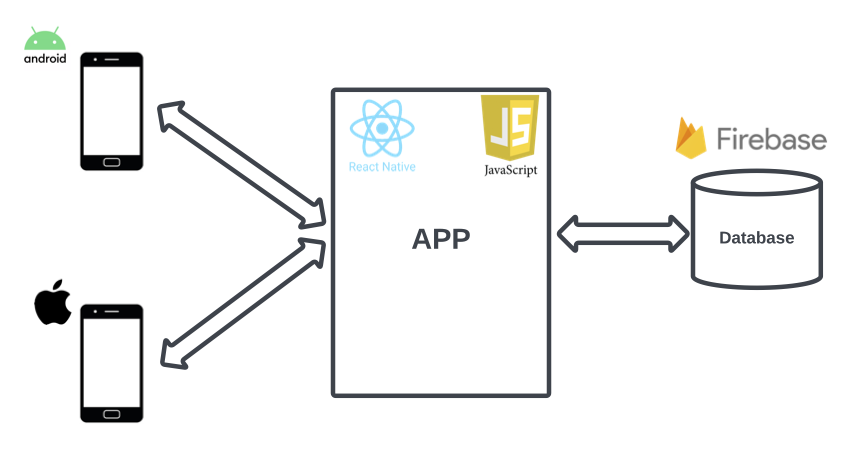
\includegraphics[width=\textwidth]{init-comp-diag.png}}
    \end{subfigure}
    \caption{Initial component diagram of architecture} 
    \label{fig:compDiag}
\end{figure}
\FloatBarrier
Here, we can see that the application code is interacting with Firebase, and then formatting this data to then be displayed to the user. The application code is also handling inputs from the user and then formatting this data to then be sent to Firebase to be stored. This is still fundamentally a model view controller architecture with separations between storing the data, interacting with this data model, and, displaying this data, but, with the controlling and displaying of data more integrated together into a more view-controller.

\section{User Interface}
\subsection*{Figma}
To design the user interface some initial sketches were drawn up and then converted into more concrete wire frames. Figma \cite{figma} an interactive interface design tool was used to create these wire frames. Figma allows the user to create high quality interface designs that can incorporate animation, leading to the creation of an initial design prototype. Through their mobile application you can visualise these design prototypes on your device, enhancing the developer experience and leading to better designs. Shown below are some initial designs that were created through Figma, and then later developed into the final application. For the full set of designs see \ref{appendix:figmaScreens}.

\begin{figure}[!htbp]
    \centering
    \begin{subfigure}[b]{0.25\textwidth}
        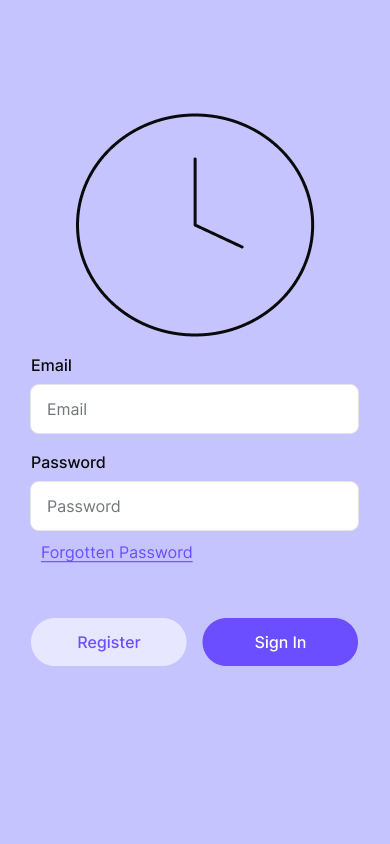
\includegraphics[width=\textwidth]{designSignIN.png}
        \caption{Sign In page}
    \end{subfigure}
    \hspace{1.5em}
    \begin{subfigure}[b]{0.25\textwidth}
        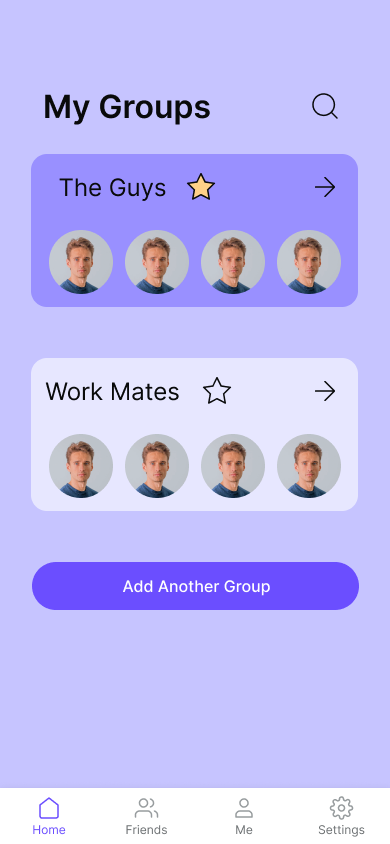
\includegraphics[width=\textwidth]{designHome.png}
        \caption{Home Page}
    \end{subfigure}
    \hspace{1.5em}
    \begin{subfigure}[b]{0.25\textwidth}
        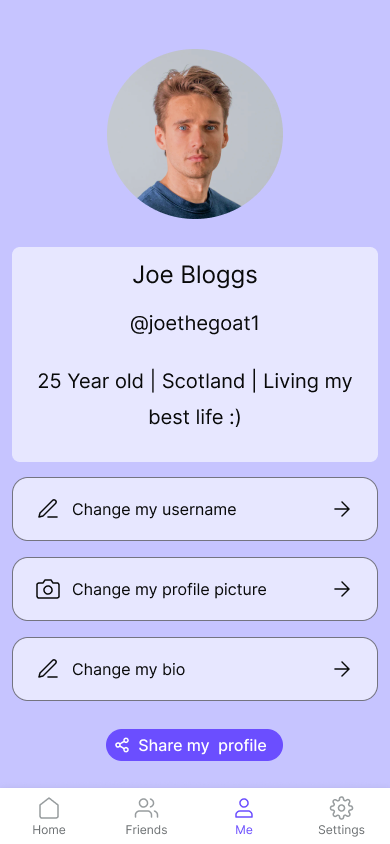
\includegraphics[width=\textwidth]{designProfile.png}
        \caption{Profile Page}
    \end{subfigure}
    \caption{Some initial screen designs from Figma}
    \label{fig:figma}
\end{figure}
\FloatBarrier

\subsection*{Design Motivations}
Having an aesthetically pleasing and highly accessible application was a must have requirement for this project as listed in \ref{functional}. This meant that a high level of detail had to be put into the initial designs to not only satisfy this requirement, but make implementation easier. Rounded corners were used throughout the app instead of sharp edges not only for aesthetics, but this has been said to reduce the cognitive load of users \cite{roundedCorners}, so this was an important concern. The colour scheme of eye catching light and dark purples is used throughout the design, with purple said to spark creativity and calm users \cite{purplePsych}. Not overwhelming the user was also a key concern with a focus on only displaying necessary information on each page so that the visual real estate is being used effectively. The ability for users to customize their experience is vital to driving user engagement \cite{customUserEng}, so enabling users to be able to upload a profile picture that can be shown in their groups, on the home page, and even on their profile along with other customization is vitally important top enhancing the user experience thus driving user engagement. 

\subsection*{App Structure}
The order in which screens are presented, and, navigated needs to be thoroughly thought through. Users should be able to easily navigate the application with screens presented in a logical, and meaningful order. The app should initially load with a minimalist splash screen (\ref{splash}), then redirect to a sign in screen once the application is loaded. When logged in the users are presented with a home screen including a bottom navigation bar to the three other main pages, friends, my profile, and, settings. This was the basic app structure that was designed with other relevant pages navigated to from these four main pages. A flowchart displaying the initial desired application, and, navigation layout is shown below. 

\begin{figure}[!htbp]
    \centering
    \begin{subfigure}[b]{0.6\textwidth}
        \frame{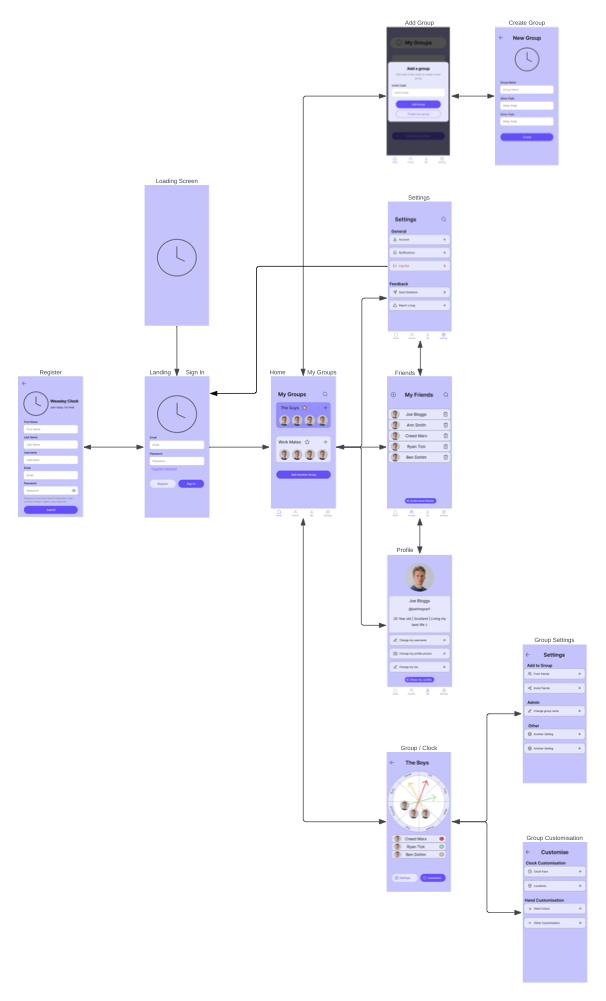
\includegraphics[width=\textwidth]{init-app-pages-flowchart.png}}
    \end{subfigure}
    \caption{Initial desired application, and, navigation layout flowchart} 
    \label{fig:layoutFlow}
\end{figure}
\FloatBarrier